%*******************************************************
% Appendix
%*******************************************************
% If problems with the headers: get headings in appendix etc. right
%\markboth{\spacedlowsmallcaps{Appendix}}{\spacedlowsmallcaps{Appendix}}

\chapter{Appenidx}

\section{Mathematica}

% \newgeometry{left=1.0in,right=1.0in}

\begin{mathematica}[ht!]
  \centering
  \captionsetup{format=plain, font=normal}
  \includegraphics[width=\linewidth, cframe=RoyalBlue 1pt]{mathematica/distance_theorem.pdf}
  \caption{Computation of probability density function for distance
    between to random points in square of side length $s$ as supplement
    to proof of Theorem~\ref{theorem:distance_square}. Note that form of
    final result \texttt{Out[7]} differs from solution given in
    \ref{theorem:distance_square}. While proof of equivalence could not
    be achieved analytically, expressions given are numerically
    equivalent, see \autoref{mathematica:comparison}.}
  \label{mathematica:distances}
\end{mathematica} 


\begin{mathematica}[t]
  \centering
  \captionsetup{format=plain, font=normal}
  \includegraphics[width=\linewidth, cframe=RoyalBlue 1pt]{%
    mathematica/distance_theorem.pdf}
  \caption{Computation of probability density function for distance
    between to random points in square of side length $s$ as supplement
    to proof of Theorem~\ref{theorem:distance_square}. Note that form of
    final result \texttt{Out[7]} differs from solut}
  \label{mathematica:comparison}
\end{mathematica} 




% ######################################################################### %
% ------------------------------------------------------------------------- %
%                 Reproducibility in Computational Research         
% ------------------------------------------------------------------------- %
% ######################################################################### %

%\section{Reproducibility in Computational Research}\label{sec:reproducibility}

%\textcite{Sumatra2012}




% ######################################################################### %
% ------------------------------------------------------------------------- %
%                         Supplementary Figures
% ------------------------------------------------------------------------- %
% ######################################################################### %

\section{Supplementary figures}\label{sec:supp_figures}

\subsection*{\autoref{ch:network_model}}

\begin{figure}[H]
  \centering
  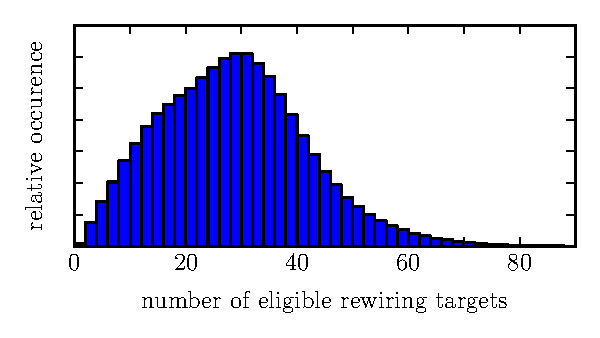
\includegraphics[width=0.8\textwidth]{%
    plots/4afc2727.pdf}
  \caption{(\smtcite{4afc2727})}
  \label{suppfig:rew_stats}
\end{figure}


\subsection*{\autoref{ch:structural_aspects}}

\begin{figure}[H]
  \centering
  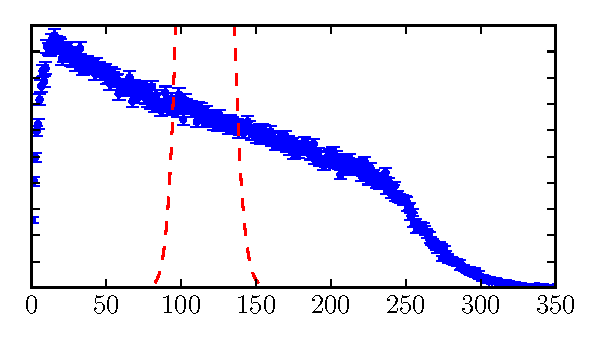
\includegraphics[width=0.7\textwidth]{%
    plots/c7ee86d7.pdf}
  \caption{(\smtcite{c7ee86d7})}
  \label{suppfig:out_degree}
\end{figure}


\begin{figure}[htp]
  \centering
  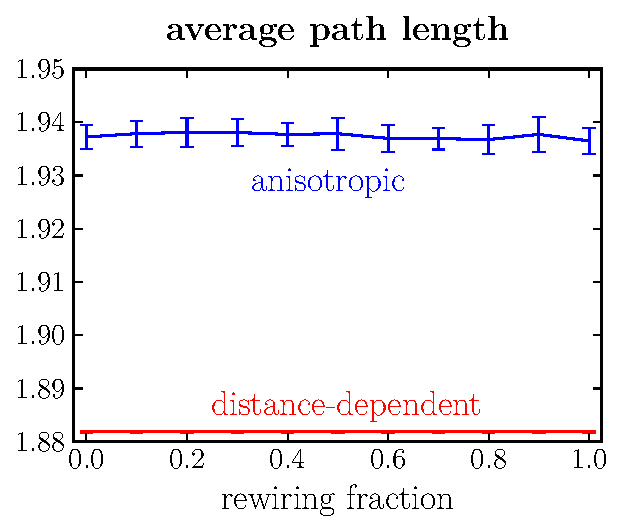
\includegraphics[width=0.5\textwidth]{plots/064f9b10_apl_1000.pdf}
  \caption{Average path length for anisotropic and distance-dependent
    networks, $N=1000$. (\smtcite{064f9b10})} %?? fix width issue!!
  \label{suppfig:small_world}
\end{figure}


\begin{figure}[htp]
  \centering
  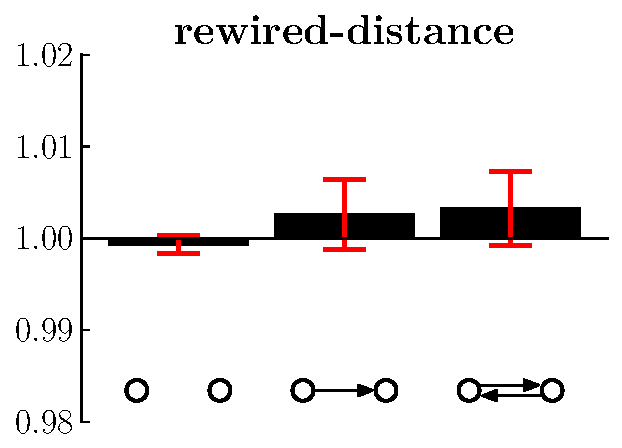
\includegraphics[width=0.5\textwidth]{plots/c5f1462b_rew_dist.pdf}
  \caption{Probabilities for connections in neuron pairs are identical
    in distance-dependent and rewired anisotropic
    networks. (\smtcite{c5f1462b})} %?? fix width issue!!
  \label{suppfig:two_neurons_dist_rew}
  \end{figure}

% \begin{figure}[H]
%   \centering
%   \includegraphics{

%%% Direct in Chapter.

% \begin{minipage}[t]{0.48\textwidth}
% \begin{align*}
% % \mathbf{P}(X=1) &    =   p_u^3  \\
% % \mathbf{P}(X=2) &    =   6 p_u p_u p_s\\
% % \mathbf{P}(X=3) &    =   3 p_u p_u p_r\\
% \mathbf{P}(X=4) &    =   3 p_s^2 p_u\\
% \mathbf{P}(X=5) &    =   3 p_s^2 p_u\\
% \mathbf{P}(X=6) &    =   6 p_s^2 p_u\\
% \mathbf{P}(X=7) &    =   6 p_s p_u p_r\\
% \mathbf{P}(X=8) &    =   6 p_s p_u p_r\\
% \mathbf{P}(X=9) &    =   3 p_r^2 p_u\\
% \end{align*}
% \end{minipage}%
% \begin{minipage}[t]{0.48\textwidth}
% \begin{equation}
% \label{eq:three_motif_full}
% \begin{aligned}
% \mathbf{P}(X=10) &   =   6 p_s^3   \\
% \mathbf{P}(X=11) &   =   2 p_s^3    \\
% \mathbf{P}(X=12) &   =   3 p_s^2 p_r\\
% \mathbf{P}(X=13) &   =   6 p_s^2 p_r\\
% \mathbf{P}(X=14) &   =   3 p_s^2 p_r\\
% \mathbf{P}(X=15) &   =   6 p_s p_r^2\\
% \mathbf{P}(X=16) &   =   p_r^3 
% \end{aligned}
% \end{equation}
% \end{minipage}


%%% Local Variables: 
%%% mode: latex
%%% TeX-master: "../dplths_document"
%%% End: 